
\section{Supplementary material for Chapter 4}

\vspace*{1cm}

\subsubsection{Forest surfaces in Europe}

\begin{table}[ht]
\centering
\caption{\textbf{Forest surfaces per ecoregion.} Areas were computed using the Global Database of Forest Cover (European Commission, 2020; accessible \href{http://data.europa.eu/89h/10d1b337-b7d1-4938-a048-686c8185b290}{here}).}
\begin{tabular}[t]{lcc}
\hline
&Surface (million ha) & Proportion (\%)\\
\hline
Mediterranean & 38.5 & 15.7 \\
Atlantic & 20.6 & 8.43 \\
Continental & 64.3 & 26.3 \\
Alpine & 37.1 & 15.2 \\
Boreal & 79.0 & 32.3 \\
Other ecoregions & 5.20 & 2.13 \\
\hline
\end{tabular}
\label{tab:forest}
\end{table}

\subsubsection{ANOVA-based variance decomposition}

% \subsection{Fractional uncertainties}

\begin{figure}[htpb]
\centering
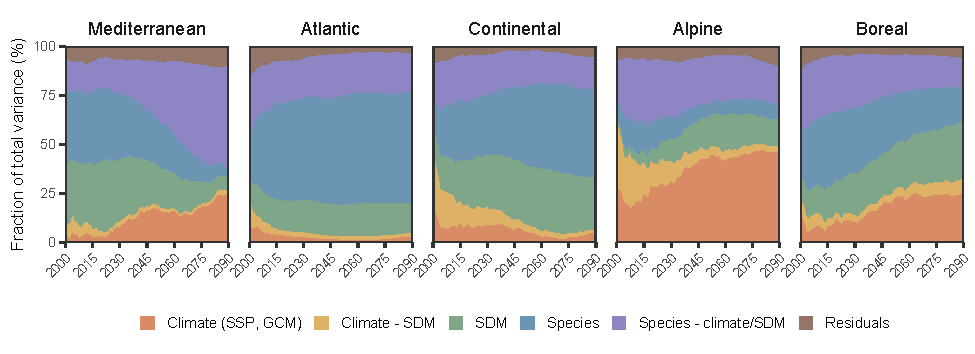
\includegraphics{chapter4/figs/appendix_frac_uncertainties-1.pdf}
\caption{\textbf{Fractional contribution of individual sources to the total uncertainty.} An ANOVA-based variance decomposition was performed to distinguish between 5 main uncertainty sources: (i) the future climate projections (GCM, SSP, and their interactions), (ii) the interactions between SDM and climate projections (both GCMs and SSPs), (iii) the modeling method (SDM class), (iv) the tree species, and (v) the interactions between species and both climate projections and SDM.}
\label{app:frac}
\end{figure}

% \subsection{Species interactions with climate and SDM method}

\begin{figure}[htpb]
\centering
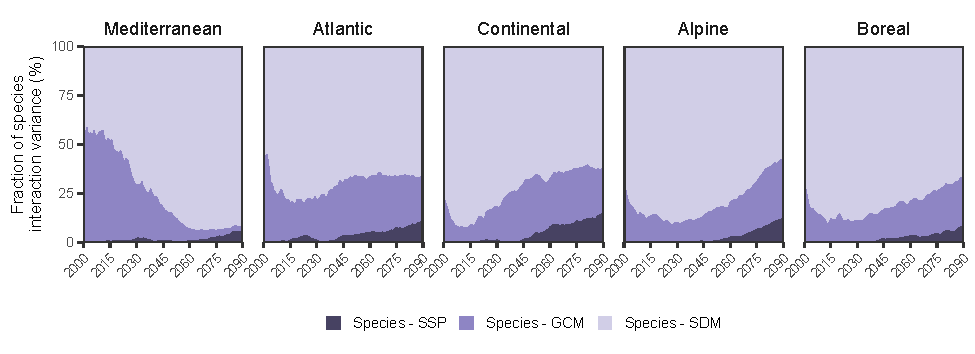
\includegraphics{chapter4/figs/appendix_speciesinteractions2-1.pdf}
\caption{\textbf{Decomposition of the contribution to the total uncertainty of the interactions between species, SSP, GCM and SDM.}}
\label{app:specinter}
\end{figure}

\begin{figure}[htpb]
\centering
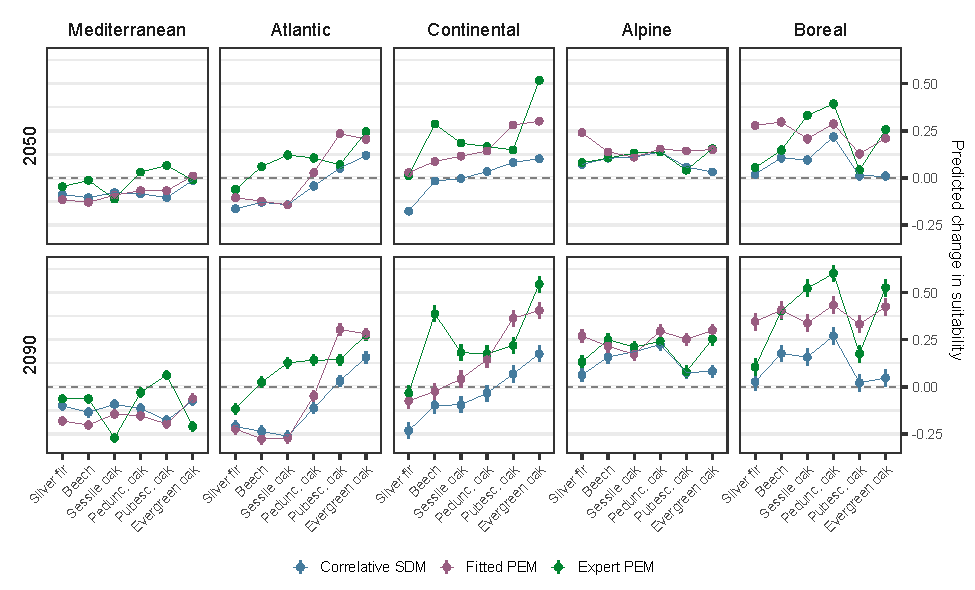
\includegraphics{chapter4/figs/appendix_speciesinteractions-1.pdf}
\caption{\textbf{Adjusted predictions of change in suitability,  for all combinations of species and model type (and their interactions).} Other predictors (GCM, SSP) are marginalized over their different levels, to represent \emph{average} conditions. See the R package \emph{ggeffects} for details.}
\label{app:spectrend}
\end{figure}

\clearpage

\subsubsection{ANOVA-based variance decomposition, only with correlative models}

\begin{figure}[htpb]
\centering
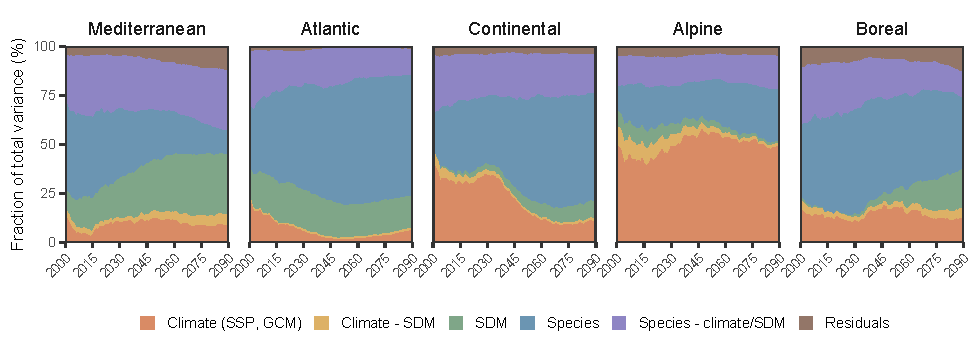
\includegraphics{chapter4/figs/anova_across_species_byecoregion_ONLYCSDM-1.pdf}
\caption{\textbf{Fractional contribution of individual sources to the total uncertainty, taking into account only correlative approach.} An ANOVA-based variance decomposition was performed to distinguish between 5 main uncertainty sources: (i) the future climate projections (GCM, SSP, and their interactions), (ii) the interactions between CSDM and climate projections (both GCMs and SSPs), (iii) the CSDM algorithm (GLM, GAM, BRT, RF), (iv) the tree species, and (v) the interactions between species and both climate projections and SDM.}
\end{figure}

\begin{figure}[htpb]
\centering
\vspace*{-0.3cm}
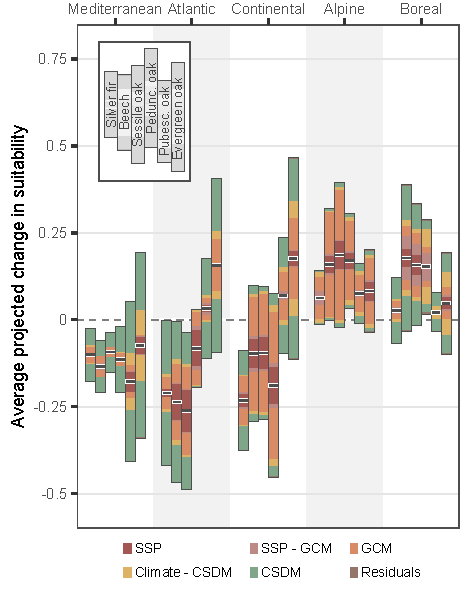
\includegraphics{chapter4/figs/anova_within_species_byecoregion_ONLYCSDM-1.pdf}
\caption{\textbf{Variance partitioning across Europe's ecoregions, for each species, taking into account only correlative approach.} An ANOVA-based variance decomposition was performed to distinguish between 5 main uncertainty sources: (i) the future scenario (SSP), (ii) the climate model used to generate the climate projections (GCM), (iii) the interactions between the SPP and the GCM, (iv) the CSDM algorithm (GLM, GAM, BRT, RF), and (v) the interactions between CSDM and climate projections (both GCMs and SSPs). The black line represents the mean projection, across all GCMs, SSPs, CSDMs and species. 90\% uncertainty ranges were calculated additively and symmetrically around the mean. Inset plot shows the species name in the same order than in the main plot.}
\label{app:anovawithinspeciesCSDM}
\vspace*{-5.2cm}
\end{figure}

\clearpage

\subsubsection{ANOVA-based variance decomposition, only with fitted models}

\begin{figure}[htpb]
\centering
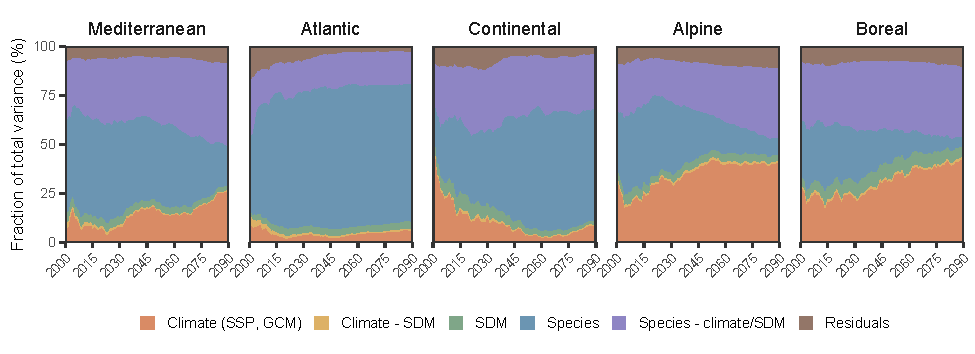
\includegraphics{chapter4/figs/anova_across_species_byecoregion_onlyhybrid-1.pdf}
\caption{\textbf{Fractional contribution of individual sources to the total uncertainty, taking into account only correlative approach.} An ANOVA-based variance decomposition was performed to distinguish between 5 main uncertainty sources: (i) the future climate projections (GCM, SSP, and their interactions), (ii) the interactions between CSDM and climate projections (both GCMs and SSPs), (iii) the repetition of the inverse calibration of the fitted PEM (FPEM), (iv) the tree species, and (v) the interactions between species and both climate projections and PEM inverse calibration.}
\end{figure}

\begin{figure}[htpb]
\centering
\vspace*{-0.3cm}
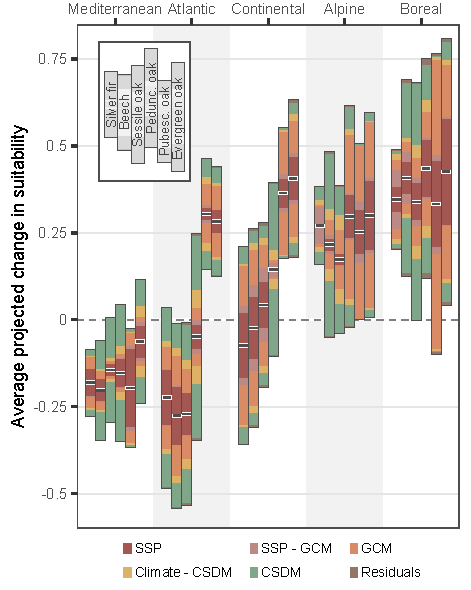
\includegraphics{chapter4/figs/anova_within_species_byecoregion_onlyhybrid-1.pdf}
\caption{\textbf{Variance partitioning across Europe's ecoregions, for each species, taking into account only correlative approach.} An ANOVA-based variance decomposition was performed to distinguish between 5 main uncertainty sources: (i) the future scenario (SSP), (ii) the climate model used to generate the climate projections (GCM), (iii) the interactions between the SPP and the GCM, (iv) the repetition of the inverse calibration of the fitted PEM (FPEM), and (v) the interactions between FPEM clibration and climate projections (both GCMs and SSPs). The black line represents the mean projection, across all GCMs, SSPs, FPEMs and species. 90\% uncertainty ranges were calculated additively and symmetrically around the mean. Inset plot shows the species name in the same order than in the main plot.}
\vspace*{-5.2cm}
\end{figure}

\clearpage

\subsubsection{Quercus robur projections}

\begin{figure}[htpb]
\centering
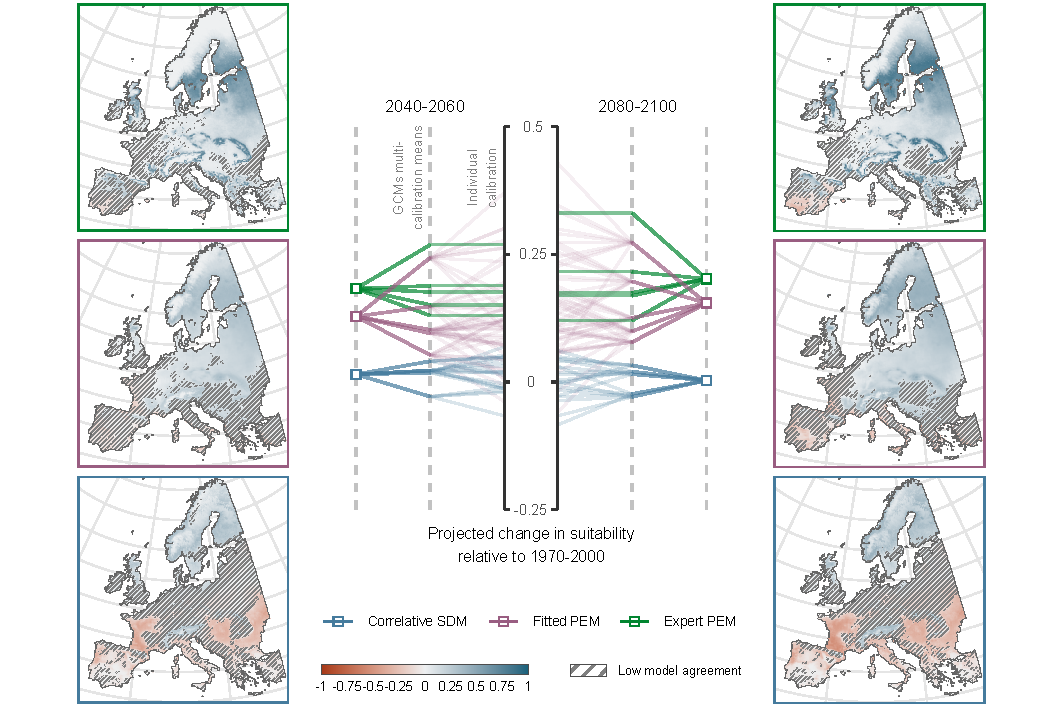
\includegraphics{chapter4/figs/quercusrobur_cascade-1.pdf}
\caption{\textbf{Discrepancies between model classes in projected future climatic suitability change for pedonculate oak.} Models are forced with climatic data from 5 GCMs under scenario SSP2-4.5. Areas with a lack of model agreement (less than 80\% of the individual calibrations agree on the sign of the change) are marked by hatching. Each individual calibrated model (i.e. 4 different CSDMs, 10 fitted PEM parameter sets, and 1 expert PEM parameter set) was run with the 5 different GCM climatic variables (i.e. 20 CSDM projections, 50 fitted PEM projections and 5 expert PEM projections). Then, they were averaged at the GCM-level within each SDM class ("GCMs multi-calibration means"), and further averaged into one ensemble per SDM class.}
\label{app:qrobproj}
\end{figure}

\begin{figure}[htpb]
\centering
\vspace*{-0.2cm}
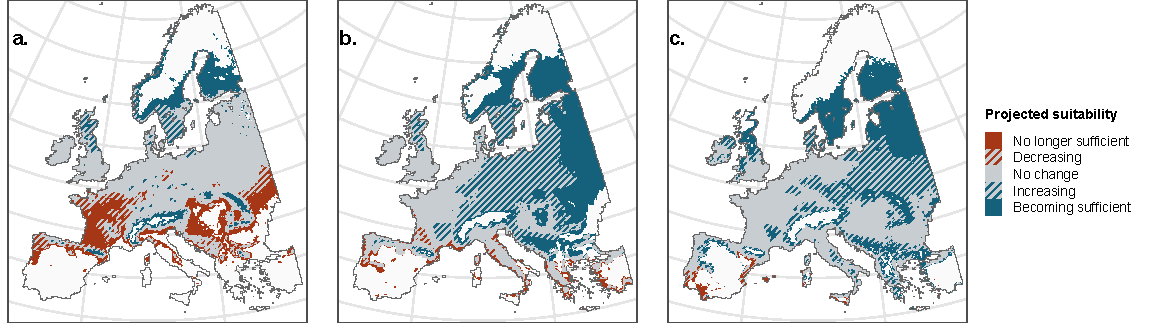
\includegraphics{chapter4/figs/quercusrobur_distributions-1.pdf}
\caption{\textbf{Projected pedonculate oak distribution in 2090, according to (a) correlative species distribution models, (b) fitted process-explicit models and (c) expert process-explicit models.} Models are forced with climatic data from 5 GCMs under scenario SSP2-4.5. For each model class, the species is considered present/absent if more than half of the simulations agree.}
\label{app:qrobdist}
\vspace*{-6cm}
\end{figure}

\clearpage

\subsubsection{Quercus petraea projections}

\begin{figure}[htpb]
\centering
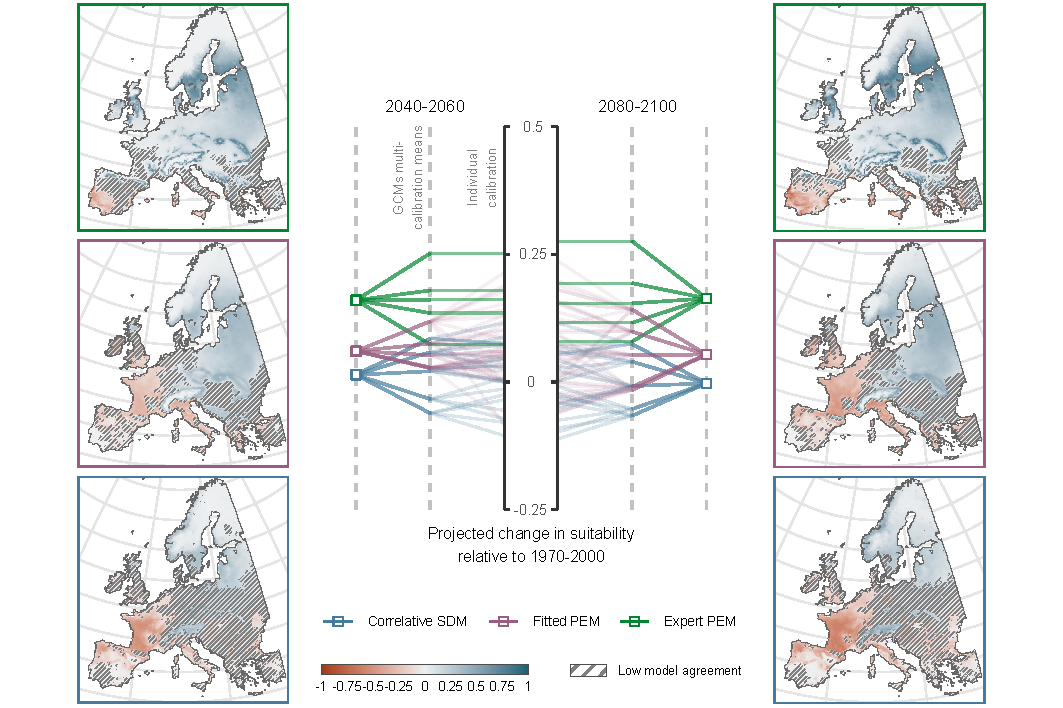
\includegraphics{chapter4/figs/quercuspetraea_cascade-1.pdf}
\caption{\textbf{Discrepancies between model classes in projected future climatic suitability change for sessile oak.} Models are forced with climatic data from 5 GCMs under scenario SSP2-4.5. Areas with a lack of model agreement (less than 80\% of the individual calibrations agree on the sign of the change) are marked by hatching. Each individual calibrated model (i.e. 4 different CSDMs, 10 fitted PEM parameter sets, and 1 expert PEM parameter set) was run with the 5 different GCM climatic variables (i.e. 20 CSDM projections, 50 fitted PEM projections and 5 expert PEM projections). Then, they were averaged at the GCM-level within each SDM class ("GCMs multi-calibration means"), and further averaged into one ensemble per SDM class.}
\label{app:qpetproj}
\end{figure}

\begin{figure}[htpb]
\centering
\vspace*{-0.2cm}
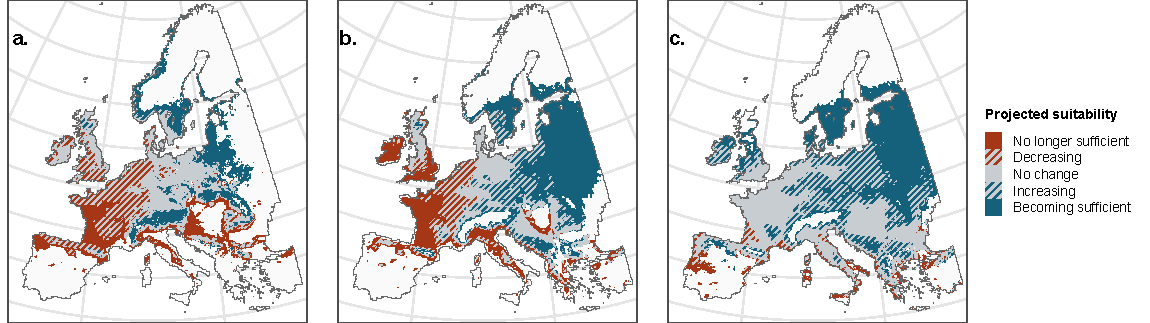
\includegraphics{chapter4/figs/quercuspetraea_distributions-1.pdf}
\caption{\textbf{Projected sessile oak distribution in 2090, according to (a) correlative species distribution models, (b) fitted process-explicit models and (c) expert process-explicit models.} Models are forced with climatic data from 5 GCMs under scenario SSP2-4.5. For each model class, the species is considered present/absent if more than half of the simulations agree.}
\label{app:qpetdist}
\vspace*{-6cm}
\end{figure}

\clearpage

\subsubsection{Quercus ilex projections}

\begin{figure}[htpb]
\centering
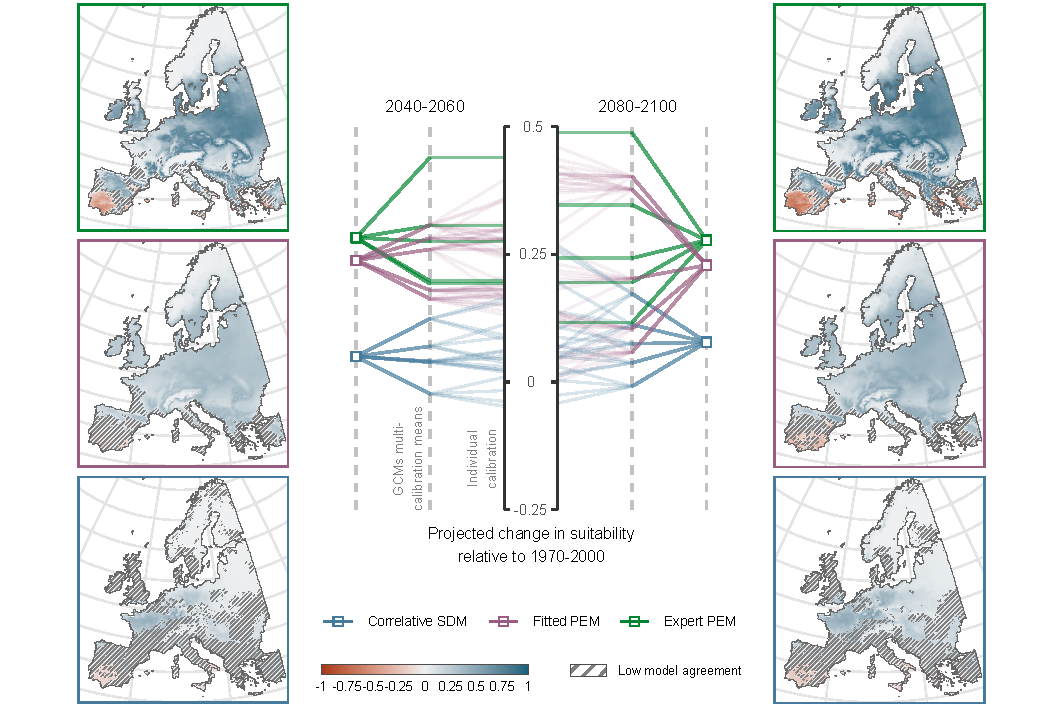
\includegraphics{chapter4/figs/quercusilex_cascade-1.pdf}
\caption{\textbf{Discrepancies between model classes in projected future climatic suitability change for evergreen oak.} Models are forced with climatic data from 5 GCMs under scenario SSP2-4.5. Areas with a lack of model agreement (less than 80\% of the individual calibrations agree on the sign of the change) are marked by hatching. Each individual calibrated model (i.e. 4 different CSDMs, 10 fitted PEM parameter sets, and 1 expert PEM parameter set) was run with the 5 different GCM climatic variables (i.e. 20 CSDM projections, 50 fitted PEM projections and 5 expert PEM projections). Then, they were averaged at the GCM-level within each SDM class ("GCMs multi-calibration means"), and further averaged into one ensemble per SDM class.}
\label{app:qileproj}
\end{figure}

\begin{figure}[htpb]
\centering
\vspace*{-0.2cm}
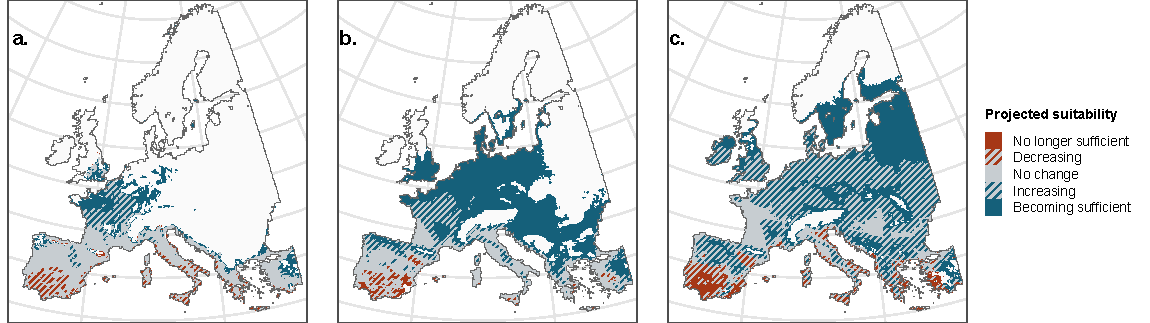
\includegraphics{chapter4/figs/quercusilex_distributions-1.pdf}
\caption{\textbf{Projected evergreen oak distribution in 2090, according to (a) correlative species distribution models, (b) fitted process-explicit models and (c) expert process-explicit models.} Models are forced with climatic data from 5 GCMs under scenario SSP2-4.5. For each model class, the species is considered present/absent if more than half of the simulations agree.}
\label{app:qiledist}
\vspace*{-6cm}
\end{figure}

\clearpage

\subsubsection{Quercus pubescens projections}

\begin{figure}[htpb]
\centering
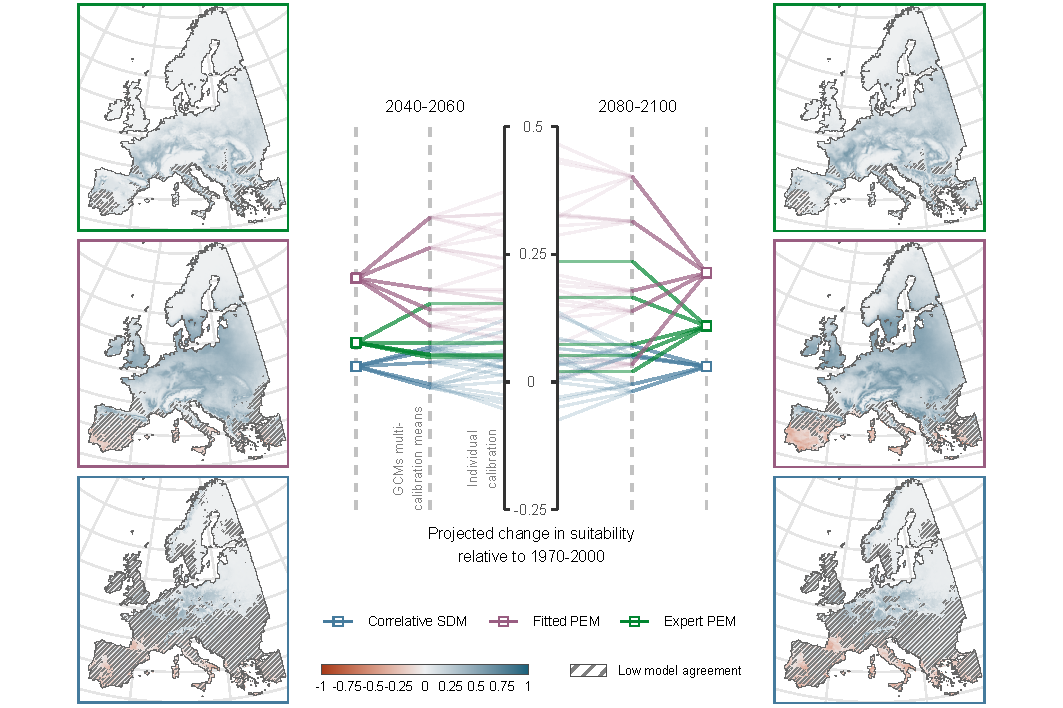
\includegraphics{chapter4/figs/quercuspubescens_cascade-1.pdf}
\caption{\textbf{Discrepancies between model classes in projected future climatic suitability change for pubescent oak.} Models are forced with climatic data from 5 GCMs under scenario SSP2-4.5. Areas with a lack of model agreement (less than 80\% of the individual calibrations agree on the sign of the change) are marked by hatching. Each individual calibrated model (i.e. 4 different CSDMs, 10 fitted PEM parameter sets, and 1 expert PEM parameter set) was run with the 5 different GCM climatic variables (i.e. 20 CSDM projections, 50 fitted PEM projections and 5 expert PEM projections). Then, they were averaged at the GCM-level within each SDM class ("GCMs multi-calibration means"), and further averaged into one ensemble per SDM class.}
\label{app:qpubproj}
\end{figure}

\begin{figure}[htpb]
\centering
\vspace*{-0.2cm}
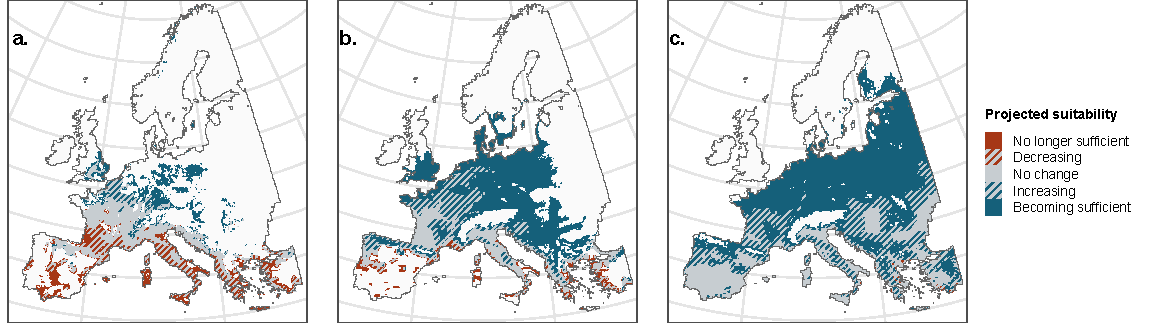
\includegraphics{chapter4/figs/quercuspubescens_distributions-1.pdf}
\caption{\textbf{Projected pubescent oak distribution in 2090, according to (a) correlative species distribution models, (b) fitted process-explicit models and (c) expert process-explicit models.} Models are forced with climatic data from 5 GCMs under scenario SSP2-4.5. For each model class, the species is considered present/absent if more than half of the simulations agree.}
\label{app:qpubdist}
\vspace*{-6cm}
\end{figure}

\clearpage

\subsubsection{Abies alba projections}

\begin{figure}[htpb]
\centering
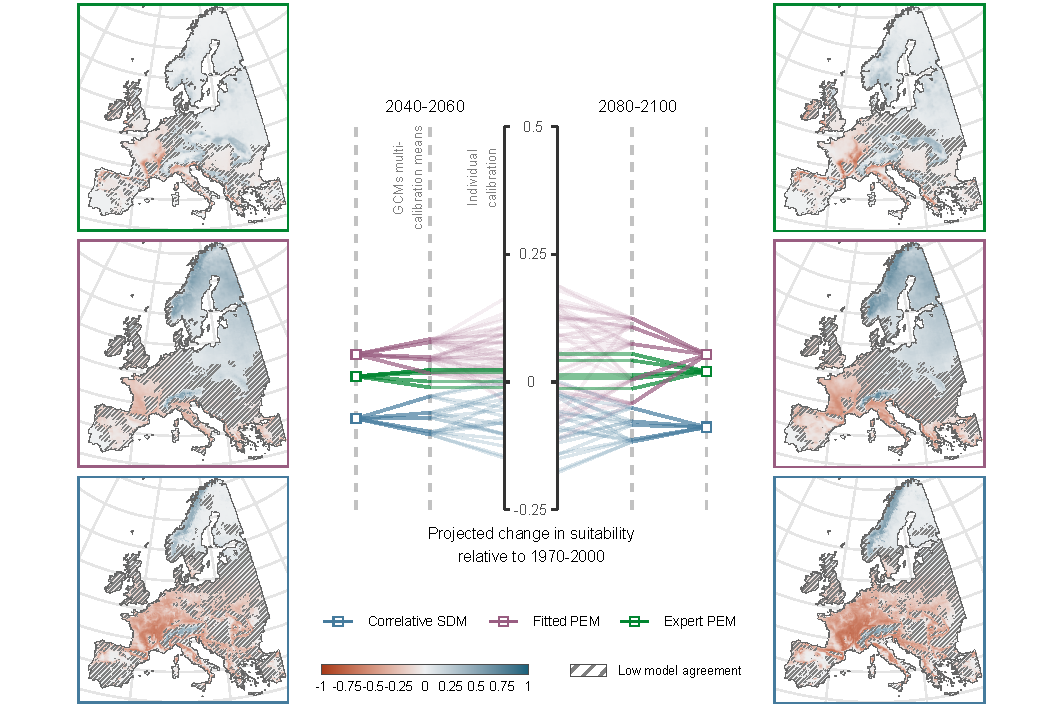
\includegraphics{chapter4/figs/abiesalba_cascade-1.pdf}
\caption{\textbf{Discrepancies between model classes in projected future climatic suitability change for fir.} Models are forced with climatic data from 5 GCMs under scenario SSP2-4.5. Areas with a lack of model agreement (less than 80\% of the individual calibrations agree on the sign of the change) are marked by hatching. Each individual calibrated model (i.e. 4 different CSDMs, 10 fitted PEM parameter sets, and 1 expert PEM parameter set) was run with the 5 different GCM climatic variables (i.e. 20 CSDM projections, 50 fitted PEM projections and 5 expert PEM projections). Then, they were averaged at the GCM-level within each SDM class ("GCMs multi-calibration means"), and further averaged into one ensemble per SDM class.}
\label{app:aalbproj}
\end{figure}

\begin{figure}[htpb]
\centering
\vspace*{-0.2cm}
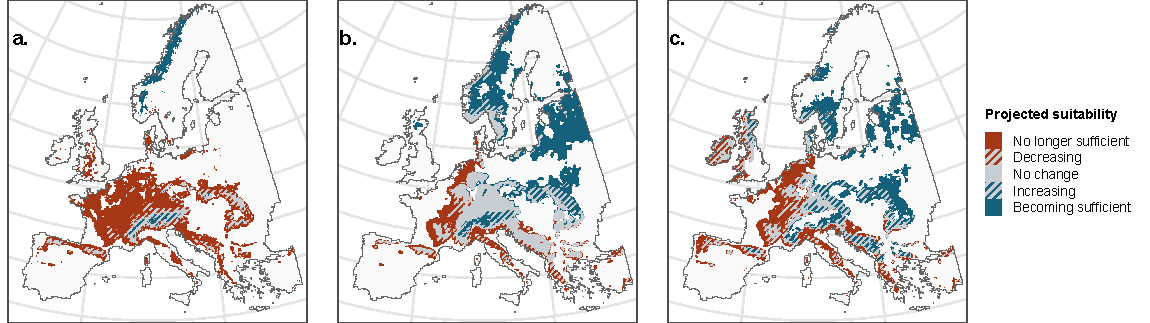
\includegraphics{chapter4/figs/abiesalba_distributions-1.pdf}
\caption{\textbf{Projected fir distribution in 2090, according to (a) correlative species distribution models, (b) fitted process-explicit models and (c) expert process-explicit models.} Models are forced with climatic data from 5 GCMs under scenario SSP2-4.5. For each model class, the species is considered present/absent if more than half of the simulations agree.}
\label{app:aalbdist}
\vspace*{-6cm}
\end{figure}